% ---------------------------------------------------------------------------
% Springer Nature "sn-jnl" class.
%   sn-basic  -> Basic Springer Nature reference style (NameDate/authoryear
%                citations by default; the class itself loads natbib with the
%                [authoryear] option and sets \bibliographystyle{sn-basic}).
%   iicol     -> required double-column layout option for this journal.
%   pdflatex  -> tells the class we are compiling with pdflatex, which skips
%                the class's own attempt to load the DVI/PS-only "breakurl"
%                package (breakurl is incompatible with pdflatex; xurl below
%                supplies the same URL-breaking behaviour under pdflatex).
% ---------------------------------------------------------------------------
\documentclass[sn-basic,iicol,pdflatex]{sn-jnl}

% ---------------------------------------------------------------------------
% Packages
% ---------------------------------------------------------------------------
% NOTE on packages removed from the original article-class preamble:
%   fontspec  - dropped. It was loaded bare (no \setmainfont/\newfontfamily
%               anywhere in the document), so nothing depends on it; dropping
%               it lets us compile with pdflatex as the class expects.
%   geometry  - dropped. sn-jnl.cls itself loads geometry with the exact A4
%               trim/margins required by the [iicol] layout; re-loading it
%               here with different options ([margin=1in]) would raise an
%               "Option clash for package geometry" error.
%   natbib    - dropped. The [sn-basic] class option already loads
%               \usepackage[authoryear]{natbib} and sets
%               \bibliographystyle{sn-basic} internally; reloading natbib
%               with [round] here would clash with the class's own load.
%   hyperref  - dropped as a \usepackage line. sn-jnl.cls unconditionally
%               \RequirePackage{hyperref}s itself; re-issuing \usepackage
%               with different options clashes, so the same options are
%               applied below via \hypersetup instead.
% xcolor and manyfoot are required by sn-jnl.cls itself (\email uses
% \textcolor, and \AtBeginDocument calls \SetFootnoteHook/\DeclareNewFootnote
% from manyfoot); they are not loaded by the class, so the document must
% supply them, exactly as sn-article.tex does.
\usepackage{xcolor}
\usepackage{manyfoot}
\usepackage{microtype}
\usepackage{graphicx}
\usepackage{amsmath,amssymb}
\usepackage{booktabs}
\usepackage{array}
\usepackage{caption}
\usepackage{subcaption}
\usepackage{float}
\usepackage{enumitem}
\usepackage{xurl}
\usepackage{setspace}
\usepackage{algorithm}
\usepackage{algpseudocode}

\hypersetup{colorlinks=true, linkcolor=black, citecolor=black, urlcolor=blue}

\newcommand{\dbar}{\ensuremath{\bar d}}

\begin{document}

\title[Deep Neural Network Surrogates for ABC in Markov Branching Processes]{\begin{tabular}[t]{@{}c@{}}\textbf{Deep Neural Network Surrogates for Approximate}\\\textbf{Bayesian Computation:}\\\textbf{A Simulation Study for Mutation-Rate Estimation}\\\textbf{in Markov Branching Processes}\end{tabular}}

\author*[1]{\fnm{Sachin} \sur{Letchumanan}}\email{sachin.letchumanan@gmail.com}
\author[1]{\fnm{Hongxiao} \sur{Zhu}}\email{hongxiao@vt.edu}
\author[1]{\fnm{Xiaowei} \sur{Wu}}\email{xwwu@vt.edu}
\affil*[1]{\orgdiv{Department of Statistics}, \orgname{Virginia Tech}, \orgaddress{\city{Blacksburg}, \state{VA}, \postcode{24061}, \country{USA}}}

\abstract{Approximate Bayesian computation (ABC) enables likelihood-free inference for stochastic simulators, but its per-iteration cost makes posterior analysis infeasible when the simulator is slow, as for the branching-process models used to estimate mutation rates from Luria--Delbr\"uck-style fluctuation experiments. A standard remedy substitutes a Gaussian-process (GP) surrogate for the simulator inside an ABC Markov chain Monte Carlo (MCMC) sampler, but a cubic fitting cost limits how much simulator output the surrogate can use. We ask whether a heteroscedastic neural-network surrogate, calibrated by split-conformal prediction, can make the same substitution, and when it helps. In the main study, a three-parameter two-stage mutation model, accuracy is governed by what the summary statistic identifies, not by the surrogate. In a tractable regime the network and the GP tie at the data's noise floor. In the regime of the original study, reached with a fast simulator that we correct and validate, the network is clearly better than a GP, even one five times larger. An amortized neural posterior estimator trained on the same simulations beats every surrogate on the well-identified parameter and cannot exceed the identifiability ceiling on the others. Coverage at fixed truths saturates at one for weakly identified parameters; simulation-based calibration over prior draws shows all methods mildly overconfident. A one-dimensional benchmark shows tighter calibrated intervals and a 68- to 2,000-fold speedup over exact ABC-MCMC. Code, data and a reproducible pipeline accompany the paper.}

\keywords{approximate Bayesian computation; likelihood-free
inference; surrogate modeling; conformal prediction; heteroscedastic
regression; Markov branching process}

\maketitle


% =============================================================================
\section{Introduction}
\label{sec:intro}
% =============================================================================

Approximate Bayesian computation (ABC) makes Bayesian inference possible for
stochastic models whose likelihood is intractable but which can be simulated
forward \citep{beaumont2002,marjoram2003,marin2012}. The basic ABC-MCMC sampler
\citep{marjoram2003} accepts a proposed parameter $\theta'$ in proportion to how
closely a simulated summary statistic matches the observed one. Every iteration
costs at least one forward simulation, so when the simulator is expensive the
per-iteration cost dominates the analysis and can put a full posterior
exploration out of reach.

\citet{lu2023} study this problem for a two-type Markov branching process (MBP)
model of microbial mutation, used to estimate mutation probabilities from
Luria--Delbr\"uck-style fluctuation experiments. Their exact simulator
(Algorithm~2) tracks the process cell by cell, and a single call takes from a
fraction of a second to several minutes. To make ABC-MCMC tractable they apply
\emph{GPS-ABC} \citep{meeds2014}: fit a Gaussian process (GP) regression
surrogate to a modest design of simulator outputs, then use the GP's predictive
mean and variance in place of the simulator inside the acceptance step. This is
the source of their reported two-to-three-order-of-magnitude speedup.

The GP brings a scaling limit that is well known and, here, binding. Fitting an
$n$-point GP costs $O(n^3)$ and a query costs $O(n)$ in the dense
implementation used at this problem size. \citet{lu2023} accordingly work with
about $50$ design points in the one-dimensional case and $1{,}500$ in their
four-parameter extension, and note that GPS-ABC can be \emph{less} accurate than
plain ABC-MCMC when the design must be built from the expensive exact simulator.
We ask:

\begin{quote}
\emph{Can a neural-network surrogate replace the Gaussian process inside the same
ABC-MCMC procedure, and under what conditions does it help?}
\end{quote}

A feedforward network has no cubic fitting term and its query cost is flat in
the size of its training set. It also gives up something the GP provides for
free: a predictive variance. Inside the ABC acceptance kernel that variance is
consumed directly, so a network must be built to produce one and then calibrated
(Section~\ref{sec:method}). That requirement, rather than the regression
itself, makes the substitution non-trivial.

\noindent\textbf{Contributions.} The paper's centre of gravity is the
multi-parameter two-stage model (Study II); the one-dimensional model
(Study I) is the benchmark that shows where a surrogate matters.
\begin{enumerate}[label=(\roman*),leftmargin=*,itemsep=2pt,topsep=2pt]
\item \emph{A calibrated neural surrogate.} A heteroscedastic network with
split-conformal calibration \citep{lei2018} that substitutes for the GP in
\citeauthor{lu2023}'s sampler with no other change to the inference algorithm.
\item \emph{Identifiability, not the surrogate, limits accuracy.} For the
two-stage model estimated jointly in $(p_1,p_2,\tau)$, the network and the GP
sit at the data's irreducible noise floor and tie on inference. Accuracy is set
by what the single summary statistic identifies: $p_2$ well, $p_1$ weakly,
$\tau$ barely. An amortized neural posterior estimator (NPE) trained on the same
simulation budget beats every surrogate, and the exact sampler, on $p_2$ and
does no better on the parameters the model cannot identify.
\item \emph{The same conclusions in the published regime.} Reaching the
parameter regime of \citeauthor{lu2023} ($t_p=20$, $p\in[10^{-11},10^{-7}]$)
requires a fast simulator. We show that the construction previously available
undercounts mutation events by about a factor of two, replace it with one
validated against the exact simulator, and repeat the two-stage study there
(Study II, Part B).
\item \emph{Calibration diagnostics that do not saturate.} Credible-interval
coverage at a fixed truth is $1.000$ for any nearly unidentified parameter
because the interval spans the prior. We replace it with simulation-based
calibration over truths drawn from the prior \citep{talts2018} together with
posterior contraction.
\item \emph{A one-dimensional benchmark.} The one setting where surrogate error
does bind: the network's input-dependent variance yields tighter,
still-calibrated intervals than the GP, and DNN-ABC is $68$ to over $2{,}000$
times faster than exact ABC-MCMC.
\item \emph{Negative results we report rather than tune away.} Convolutional and
recurrent surrogates do not improve on the feedforward one, and network capacity
beyond roughly $700$ parameters buys nothing once the noise floor is reached.
\end{enumerate}

\noindent\textbf{Related work.} GPS-ABC is one instance of a line of work using
Gaussian processes to reduce simulator calls in likelihood-free inference:
\citet{wilkinson2014} models the ABC log-likelihood surface directly,
\citet{gutmann2016}'s BOLFI uses Bayesian optimization to place the next
expensive simulation, and \citet{jarvenpaa2021,jarvenpaa2023} extend this to
noisy, parallel and predictive settings. All inherit the $O(n^3)$ fitting cost;
none substitutes a neural surrogate for the GP, which is the substitution
studied here. A separate literature avoids the GP-versus-network choice by
learning the posterior (or likelihood, or likelihood ratio) directly with a
neural density estimator trained on simulator draws
\citep{papamakarios2016,greenberg2019,cranmer2020}, implemented in toolkits such
as \texttt{sbi} \citep{tejerocantero2020}. These methods are \emph{amortized}:
training is paid once and new data sets need no further simulation or MCMC,
which GPS-ABC, DNN-ABC and exact ABC-MCMC cannot offer. We include NPE in Study
II to make that trade-off concrete, there rather than in Study I because Study
II is the only setting with both a well-identified and weakly identified
parameter estimated jointly, the contrast that makes the amortized-versus-surrogate
question informative. The coverage question is motivated by
\citet{talts2018} and \citet{hermans2022}, who report that posterior
approximations routinely pass regression-level diagnostics yet fail to cover the
truth at the stated rate when checked directly, and by \citet{fanwhite2026},
who show that a narrow NPE proposal can give a biased posterior that still
reproduces the observed summaries. Section~\ref{sec:sim1D_coverage}'s distinction
between the surrogate's regression coverage and the ABC posterior's coverage is
an instance of the same failure mode.

The paper proceeds as follows. Section~\ref{sec:background} reviews the model
and GPS-ABC, Section~\ref{sec:method} develops the surrogate, and
Sections~\ref{sec:sim1D} and \ref{sec:sim3D} report the two studies.
Section~\ref{sec:discussion} discusses implications and limitations and
Section~\ref{sec:repro} describes the reproducible pipeline.

% =============================================================================
\section{Background: ABC for the Markov Branching Process Model}
\label{sec:background}
% =============================================================================

\subsection{The mutation model and the observed statistic}

Following \citet{lu2023}, a population initiated by a single wild-type cell
grows for a fixed observation period under a two-type Markov branching process
(MBP). Three quantities govern it: the per-division mutation probability $p$,
the division-rate parameter $a$ (which sets the time scale), and the mutant
relative growth rate $\delta$. We take $a=\delta=1$ throughout, as they do in
every figure and data analysis. We refer to \citet{lu2023} for the full
construction and for their Algorithm~2 (an exact, cell-by-cell simulator) and
Algorithm~4 (a fast approximate simulator). We re-implement both in Python;
Section~\ref{sec:validation} validates the exact port against their R/MATLAB
code, and Section~\ref{sec:fastsim} shows that the fast simulator must be
rebuilt before it can be used.

An experiment consists of $J$ independently plated parallel cultures, each
grown from one wild-type cell for the same fixed time. Culture $j$ yields a
final wild-type count $Z_j$ and mutant count $X_j$. Following
\citeauthor{lu2023}, we work with the scalar summary
\[
\dbar \;=\; \frac{1}{J}\sum_{j=1}^{J} \sqrt{X_j / Z_j},
\]
and, for the two-stage model, its fourth-root analogue (Section~\ref{sec:groundtruth3D}).
Every regression below models $\log_{10}\dbar$ rather than $\dbar$, because
$\log_{10}\dbar$ varies smoothly and close to linearly in $\theta \equiv
\log_{10} p$ (\citealp{lu2023}, Figure~2), a target both GP and neural-network
regression fit considerably better.

\subsection{ABC-MCMC and GPS-ABC}
\label{sec:abcmcmc}

Write $\theta = \log_{10} p$. Given an observed statistic $\dbar_{\mathrm{obs}}$,
classical ABC-MCMC \citep{marjoram2003} targets
\[
\pi_\epsilon(\theta \mid \dbar_{\mathrm{obs}}) \;\propto\; \pi(\theta)\,
\mathbb{E}_{S \sim F_\theta}\!\left[K_\epsilon\!\left(\dbar_{\mathrm{obs}}, S\right)\right],
\]
with a smoothing kernel $K_\epsilon$ of bandwidth $\epsilon$. The ``exact''
baseline throughout this paper is not this literal kernel average but Wood's
\citep{wood2010} \emph{synthetic likelihood}: at each proposed $\theta'$ we draw
$n_s$ pilot simulations, take their sample mean $m(\theta')$ and variance
$v(\theta')$, and score $\dbar_{\mathrm{obs}}$ against a matched Gaussian,
\[
\hat\pi_\epsilon(\dbar_{\mathrm{obs}} \mid \theta') \;=\;
\mathcal{N}\!\left(\dbar_{\mathrm{obs}};\; m(\theta'),\; \epsilon^2 + v(\theta')\right).
\]
This is exactly the likelihood form the surrogates use, with a predicted
variance $\sigma_\phi(\theta')^2$ in place of $v(\theta')$, so every column of
the result tables shares one likelihood and differs only in how
$(m(\theta), v(\theta))$ is obtained. Algorithm~\ref{alg:abcmcmc} states the
shared Metropolis--Hastings sampler: a truncated-exponential prior on $\theta$
(uniform in the multi-parameter study) and a truncated-normal random-walk
proposal.

\begin{algorithm}[H]
\caption{ABC-MCMC (Metropolis--Hastings, synthetic likelihood)}
\label{alg:abcmcmc}
\begin{algorithmic}[1]
\State Initialize $\theta_0$; set tolerance $\epsilon$, simulator-repeat count $n_s$.
\For{$t = 1, \dots, T$}
  \State Propose $\theta' \sim q(\cdot \mid \theta_{t-1})$ (truncated-normal random walk)
  \State Obtain $(m(\theta'), v(\theta'))$: either (a) simulate $n_s$ times from $F_{\theta'}$ and take their sample mean and variance, or (b) evaluate a surrogate's predicted mean and variance $(\mu_\phi(\theta'), \sigma_\phi(\theta')^2)$ (Section~\ref{sec:method})
  \State Compute acceptance probability
  \[
  \resizebox{0.95\linewidth}{!}{$\displaystyle\alpha \;=\; \min\!\left(1,\; \frac{\pi(\theta')\,q(\theta_{t-1}\mid\theta')}{\pi(\theta_{t-1})\,q(\theta'\mid\theta_{t-1})}\,\cdot\,\frac{\hat\pi_\epsilon(\dbar_{\mathrm{obs}} \mid \theta')}{\hat\pi_\epsilon(\dbar_{\mathrm{obs}} \mid \theta_{t-1})}\right)$}
  \]
  \State Set $\theta_t = \theta'$ with probability $\alpha$, else $\theta_t = \theta_{t-1}$
\EndFor
\State \Return $\{\theta_t\}_{t=B+1}^{T}$ after discarding $B$ burn-in draws
\end{algorithmic}
\end{algorithm}

Step 4(a) is the expensive one. \emph{GPS-ABC} \citep{meeds2014}, applied by
\citet{lu2023} to this model, instead fits a GP to a design
$\{(\theta_i, \dbar_i)\}_{i=1}^n$ of simulator outputs \emph{once}, and at every
iteration uses step 4(b): the GP's predictive mean and variance replace
$(m(\theta'), v(\theta'))$ directly. This sets the standard any replacement
must meet. It is not enough to predict the mean accurately; the variance must
also be calibrated, because the two failure modes are asymmetric and both
corrupt the posterior. An overconfident $\sigma$ inflates the acceptance rate
where the surrogate does not know the response, and an underconfident one
over-rejects.

The GP's fitting cost is $O(n^3)$ and its per-query cost $O(n)$, since the
predictive mean and variance require solving a system with the full training
kernel matrix. \citet{lu2023} report about $50$ design points in the
one-dimensional case and $1{,}500$ initial points in a four-parameter extension,
and note that GPS-ABC trained on the exact simulator can be less accurate than
uncorrected ABC-MCMC, plausibly because the cubic cost forces a small design
when each design point comes from the expensive exact simulator.

% =============================================================================
\section{A Neural-Network Surrogate for ABC}
\label{sec:method}
% =============================================================================

We replace the GP in step 4(b) of Algorithm~\ref{alg:abcmcmc} with a neural
network $f_\phi$ trained to predict both the mean and the variance of
$\log_{10}\dbar$ as a function of the parameters of interest. The substitution
is deliberately minimal: the sampler, the acceptance ratio and the convolution
with $\epsilon^2$ are exactly those of GPS-ABC, so any difference in the results
is attributable to the surrogate. We call the procedure \emph{DNN-ABC}. The two
ingredients that let the network stand in for the GP are an input-dependent
predictive variance and a guarantee that it is calibrated.

\subsection{Heteroscedastic regression}
\label{sec:hetero}

$f_\phi$ has two output heads, $\mu_\phi(x)$ and $\log\sigma^2_\phi(x)$, where
$x$ is $\theta=\log_{10}p$ alone (Study I) or $(\log_{10}p_1, \log_{10}p_2,
\tau)$ (Study II), with no derived features. Both heads are trained jointly by
minimizing the Gaussian negative log-likelihood
\begin{equation}
\label{eq:nll}
\mathcal{L}(\phi) \;=\; \frac{1}{n}\sum_{i=1}^n \left[
\frac{\left(y_i - \mu_\phi(x_i)\right)^2}{2\,\sigma_\phi^2(x_i)}
\;+\; \frac{1}{2}\log \sigma_\phi^2(x_i)
\right],
\end{equation}
with $y_i = \log_{10}\dbar_i$. Unlike squared-error training, this targets an
\emph{input-dependent} predictive variance, the network's analogue of the GP's
posterior variance. That is a requirement, not a refinement: the
replicate-to-replicate noise in $\log_{10}\dbar$ is far from homoscedastic
(Sections~\ref{sec:sim1D} and \ref{sec:arch3D}), and a GP with a single noise
term cannot represent that shape.

\subsection{Split-conformal calibration}
\label{sec:conformal}

A trained variance head approximates the true conditional variance from a
finite sample; nothing in Eq.~\eqref{eq:nll} guarantees it is calibrated. Since
the acceptance step consumes it directly, we apply split-conformal calibration
\citep{lei2018}. On a held-out calibration split of size $m$ we form scores
\[
s_i \;=\; \frac{\left|y_i - \mu_\phi(x_i)\right|}{\sigma_\phi(x_i)}, \qquad i=1,\dots,m,
\]
and set the calibration factor $\hat c$ to the $\lceil (m+1)(1-\alpha)
\rceil / m$ empirical quantile of $\{s_i\}$. The calibrated $(1-\alpha)$
predictive interval is $\mu_\phi(x) \pm \hat c\, \sigma_\phi(x)$, and for
exchangeable calibration and test points it has marginal coverage of at least
$1-\alpha$ in finite samples, with no distributional assumption \citep{lei2018}.
We use $\alpha = 0.05$ and call this the surrogate's \emph{regression
calibration}, to distinguish it from the empirical coverage of the downstream
ABC credible intervals, a different quantity with no equivalent guarantee
(Sections~\ref{sec:sim1D_coverage} and \ref{sec:sim3D_sbc}). The calibrated
$\hat c\,\sigma_\phi(x)$ is also what enters the acceptance kernel, so the
uncertainty that is validated is the uncertainty the sampler uses.

\subsection{Simulator validation}
\label{sec:validation}

Ground truth is generated by re-implementations of the simulators of
\citet{lu2023}, and every number below rests on them. The exact port is
validated in two ways: the closed-form plating-time equation is solved and
compared with the R implementation's solver (agreement to $3\times10^{-5}$), and
simulated $\dbar$ means are compared against the committed ground-truth CSV at
matched grid points. The two-stage exact simulator is additionally checked
against the reference MATLAB code and, because setting $p_1=p_2$ reduces it to
the constant-rate model, against the constant-rate simulator in distribution.
The fast simulator is treated separately in Section~\ref{sec:fastsim}.

\subsection{Simulation design and reporting}
\label{sec:ademp}

We follow the ADEMP structure of \citet{morris2019}. \emph{Aims}: compare MOM,
MLE, exact ABC-MCMC, GPS-ABC and DNN-ABC in Study I, and the surrogate methods,
exact ABC-MCMC and NPE in Study II (the constant-rate MOM and MLE do not apply
there), on point accuracy, interval precision, calibration and cost.
\emph{Data-generating mechanisms}: the validated simulators, at the parameter
grids of Sections~\ref{sec:sim1D_results} and \ref{sec:sim3D_abc}.
\emph{Estimands}: $p$ (via $\theta=\log_{10}p$) in Study I and $(p_1,p_2,\tau)$
jointly in Study II. \emph{Performance measures}: MSE and normalized RMSE of
$\hat p$, mean 95\% credible-interval length, empirical coverage, and wall-clock
time per 100 MCMC iterations; for Study II also SBC coverage and posterior
contraction (Section~\ref{sec:sim3D_sbc}).

Each cell is evaluated over $R$ independent replicated data sets ($R=40$ in
Study I, $R=16$ per truth triple in Study II). Every comparison carries its
Monte Carlo standard error: for $e_r = (\hat p_r - p)^2$,
$\widehat{\mathrm{MCSE}} = \mathrm{sd}(e_r)/\sqrt{R}$. For two methods we report
the MSE gap in units of its combined MCSE (the $\Delta/\mathrm{SE}$ column of
Table~\ref{tab:mse1D}). This is a descriptive diagnostic of whether a point
comparison is resolved at the replicate count, not a hypothesis test; we call a
difference resolved when $|\Delta/\mathrm{SE}|>2$.

% =============================================================================
\section{Study I: A Benchmark with One Parameter}
\label{sec:sim1D}
% =============================================================================

Study I reproduces \citeauthor{lu2023}'s constant-rate benchmark: $a=\delta=Z_0=1$
and only $p$ varying. Its role in this paper is to show \emph{where} a surrogate
matters; the multi-parameter inference question is Study II. Ground truth is
$101$ log-spaced values of $p$ with $\log_{10}p \in [-8,-2]$, ten replicates each
($1{,}010$ rows), $J=100$. We split \emph{by replicate} rather than by grid
point, so every $p$ appears in every split and a split tests generalisation to
fresh noise, with no leakage: replicates 1--5 train ($505$ rows), 6--8 calibrate
and early-stop ($303$), 9--10 are held out ($202$). The GPS-ABC baseline is fit
on replicates 1--8, so both surrogates see the same data and neither sees the
test replicates.

The ABC comparison evaluates observed data sets at $J \in \{10, 50, 100\}$
cultures. Both surrogates are trained separately for each $J$: for $J \in
\{10, 50\}$ a $J$-culture $\dbar$ is rebuilt from the same simulated data by
averaging a random $J$-subset of the $100$ recorded per-culture values (five
subsets per row), so no new simulator calls are needed.
Section~\ref{sec:sim1D_coverage} shows why this matters.

\subsection{Architecture}
\label{sec:arch1D}

The network is a shallow funnel MLP: input $\theta=\log_{10}p$, two
GELU-activated dense layers of width $32$ and $16$ ($626$ parameters), and the
two linear heads of Section~\ref{sec:hetero}. It is trained with Adam under
early stopping on calibration-split NLL, weight decay $10^{-5}$ and no dropout.
The width is the outcome of a two-stage search (activation and normalisation at
a $128$--$64$ baseline, then capacity); full tables are in Supplementary
Material S1.

The one decisive finding is BatchNorm \citep{ioffe2015}: an otherwise reasonable
$128$--$64$ network carrying it fits \emph{eleven times worse} than the same
network without it. BatchNorm's per-minibatch statistics inject batch-dependent
noise and bias predictions near the hard edge of the one-sided $\theta$ domain,
so what closes the gap to the GP is removing a component most practitioners
include by default. Among BatchNorm-free networks, ReLU, SiLU
\citep{elfwing2018}, GELU \citep{hendrycks2016} and tanh are within $7\%$ of one
another (three seeds), a statistical tie; we choose GELU on structural grounds
(smoothness, no dead units). A second round with $7$-network deep ensembles did
not improve on the single network.

Capacity is also nearly irrelevant. A width and depth sweep from $128$--$64$ down
to a linear control (three seeds, then confirmed at paper scale: $40$ replicates,
the full $p\times J$ grid, $600$ MCMC iterations) finds $32$--$16$ the best point
estimate on curve fit and on the downstream task at $14\times$ fewer parameters,
though that margin is not distinguishable from Monte Carlo noise. Every candidate
from $8$ to $128$--$64$ parameters beats the GP baseline, and only the linear
control shows a clear cost. We therefore deploy $32$--$16$ on parsimony, and
report every table and figure below for it; the $128$--$64$ network remains in
Supplementary Material S1 as the architecture the BatchNorm search ran against.
Convolutional and recurrent architectures are not tested here: with one scalar
input a 1-D convolution has no neighbours to convolve over and a recurrent cell
no second step, so both collapse to a linear map. Study II tests them where they
are not vacuous (Section~\ref{sec:sim3D_arch}).

\subsection{Regression calibration}
\label{sec:sim1D_calib}

Table~\ref{tab:fit1D} reports the surrogate's fit and split-conformal coverage
by split.


\begin{table*}[t]
\centering
\caption{One-dimensional surrogate: fit and 95\% regression coverage by split.}
\label{tab:fit1D}
\begin{tabular}{lrrrr}
\toprule
Split & $n$ & MSE($\log_{10}\dbar$) & MAE($\log_{10}\dbar$) & 95\% coverage \\
\midrule
Train & 505 & 0.00424 & 0.0515 & 0.964 \\
Calibration & 303 & 0.00533 & 0.0538 & 0.954 \\
\textbf{Test} & \textbf{202} & \textbf{0.00434} & \textbf{0.0525} & \textbf{0.9554} \\
\bottomrule
\end{tabular}
\end{table*}

Held-out coverage of $0.9554$ ($193$ of $202$ points) is within sampling noise
of the nominal $0.95$, as the guarantee of \citet{lei2018} predicts.
Figure~\ref{fig:calib1D} shows the calibrated band and compares the network's
input-dependent predictive standard deviation with the GP's flat one.


\begin{figure*}[t]
\centering
\begin{subfigure}{0.48\textwidth}
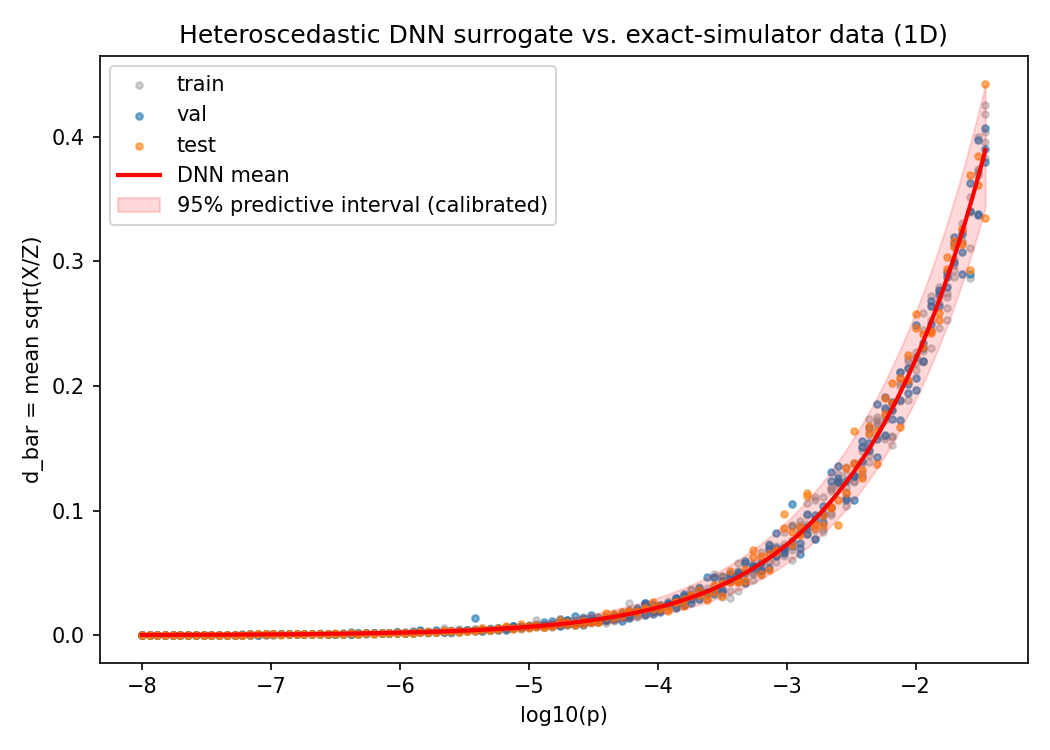
\includegraphics[width=\linewidth]{Models/1D/results/figures/surrogate_fit.png}
\caption{Calibrated 95\% predictive band}
\end{subfigure}\hfill
\begin{subfigure}{0.48\textwidth}
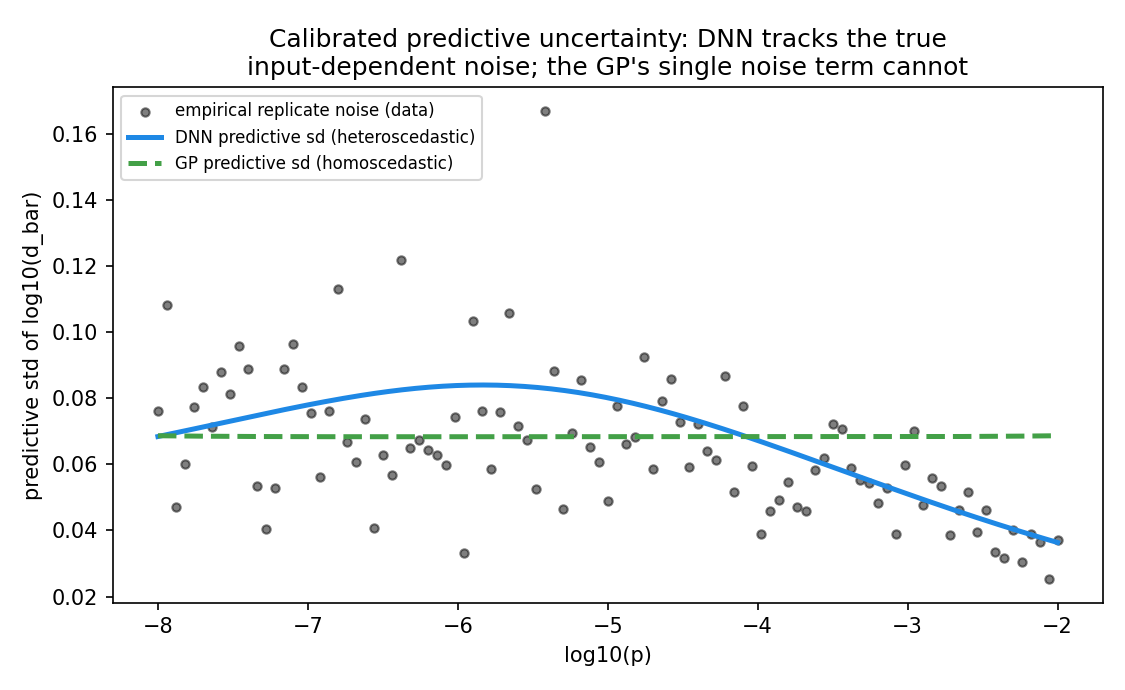
\includegraphics[width=\linewidth]{Models/1D/results/figures/fig_uncertainty.png}
\caption{Input-dependent uncertainty vs.\ the GP}
\end{subfigure}
\caption{One-dimensional surrogate calibration. Left: the calibrated 95\%
predictive band tracks the response curve across the full range of $\theta$.
Right: the network's heteroscedastic predictive standard deviation (which
enters the ABC acceptance kernel directly) tracks the true input-dependent
replicate noise, while the GP's single homoscedastic noise term is flat by
construction.}
\label{fig:calib1D}
\end{figure*}

\subsection{ABC simulation results}
\label{sec:sim1D_results}

We ran the ABC-MCMC / GPS-ABC / DNN-ABC comparison at $40$ replicated data sets
per cell, $600$ MCMC iterations ($250$ burn-in), $n_s=6$ simulator repeats per
exact iteration, and prior $\theta \sim \mathrm{TruncExp}$ on $[-5,-2]$ (bounded
so the exact simulator in the loop stays feasible; the surrogates are trained on
$[-8,-2]$ and queried in range), on the grid $p \in \{10^{-4}, 10^{-3},
10^{-2}\} \times J \in \{10, 50, 100\}$. MOM and MLE follow \citeauthor{lu2023}'s
closed forms as classical baselines.


\begin{table*}[t]
\centering
\caption{Study I, Table 1: MSE of $\hat p$ across five estimators; normalized
RMSE $\sqrt{\mathrm{MSE}}/p$ in parentheses. Bold marks the lower of GPS-ABC
and DNN-ABC in each row. $\Delta/\mathrm{SE}$ is the GPS-ABC$-$DNN-ABC MSE gap
in units of its combined Monte Carlo standard error (Section~\ref{sec:ademp});
values below $\sim 2$ in magnitude are not clearly resolved at $R=40$
replicates.}
\label{tab:mse1D}
{\small
\begin{tabular}{rrrrrrrr}
\toprule
$p$ & $J$ & MOM & MLE & ABC-MCMC & GPS-ABC & DNN-ABC & $\Delta/\mathrm{SE}$ \\
\midrule
$10^{-4}$ & 10  & 9.36e-9 (0.97) & 1.02e-8 (1.01) & 5.95e-9 (0.77) & 7.01e-9 (0.84) & \textbf{5.25e-9 (0.72)} & 0.37 \\
$10^{-4}$ & 50  & 8.68e-9 (0.93) & 9.59e-9 (0.98) & 1.91e-9 (0.44) & 1.98e-9 (0.45) & \textbf{1.77e-9 (0.42)} & 0.45 \\
$10^{-4}$ & 100 & 4.18e-9 (0.65) & 4.64e-9 (0.68) & 7.75e-10 (0.28) & 7.95e-10 (0.28) & \textbf{7.68e-10 (0.28)} & 0.10 \\
$10^{-3}$ & 10  & 1.38e-6 (1.17) & 1.60e-6 (1.26) & 4.11e-7 (0.64) & 6.46e-7 (0.80) & \textbf{4.58e-7 (0.68)} & 0.60 \\
$10^{-3}$ & 50  & 3.21e-7 (0.57) & 3.85e-7 (0.62) & 1.11e-7 (0.33) & \textbf{1.11e-7 (0.33)} & 1.33e-7 (0.36) & $-$0.48 \\
$10^{-3}$ & 100 & 2.71e-7 (0.52) & 3.29e-7 (0.57) & 4.29e-8 (0.21) & 4.48e-8 (0.21) & \textbf{4.42e-8 (0.21)} & 0.04 \\
$10^{-2}$ & 10  & 3.42e-5 (0.58) & 4.40e-5 (0.66) & 1.67e-5 (0.41) & \textbf{1.77e-5 (0.42)} & 2.30e-5 (0.48) & $-$1.02 \\
$10^{-2}$ & 50  & 7.71e-6 (0.28) & 1.17e-5 (0.34) & 7.01e-6 (0.26) & \textbf{5.46e-6 (0.23)} & 9.93e-6 (0.32) & $-$1.44 \\
$10^{-2}$ & 100 & 4.01e-6 (0.20) & 6.08e-6 (0.25) & 3.05e-6 (0.17) & \textbf{3.14e-6 (0.18)} & 3.37e-6 (0.18) & $-$0.21 \\
\bottomrule
\end{tabular}}
\end{table*}

DNN-ABC's point estimate is lower than GPS-ABC's in five of nine cells and
higher in four, but no difference in either direction is resolved: the largest
$|\Delta/\mathrm{SE}|$ is $1.44$ ($p=10^{-2}$, $J=50$, favouring GPS-ABC). This
is a statistical tie in every cell, consistent with a GP on a comparable design
already being close to optimal for a one-dimensional smooth curve. Both
surrogates match, and in several cells slightly improve on, exact ABC-MCMC, and
all ABC methods substantially outperform MOM and MLE, reproducing
\citeauthor{lu2023}'s central finding.


\begin{table*}[t]
\centering
\caption{Study I, Table 2: mean length of the 95\% ABC credible interval for
$\hat p$. Bold marks the shorter of GPS-ABC and DNN-ABC.}
\label{tab:ci1D}
\begin{tabular}{rrrrr}
\toprule
$p$ & $J$ & ABC-MCMC & GPS-ABC & DNN-ABC \\
\midrule
$10^{-4}$ & 10  & 2.62e-4 & 3.11e-4 & \textbf{2.45e-4} \\
$10^{-4}$ & 50  & 1.56e-4 & 1.50e-4 & \textbf{1.44e-4} \\
$10^{-4}$ & 100 & 1.21e-4 & 1.16e-4 & \textbf{1.16e-4} \\
$10^{-3}$ & 10  & 2.80e-3 & 3.32e-3 & \textbf{2.45e-3} \\
$10^{-3}$ & 50  & 1.43e-3 & 1.66e-3 & \textbf{1.29e-3} \\
$10^{-3}$ & 100 & 9.70e-4 & 1.20e-3 & \textbf{8.81e-4} \\
$10^{-2}$ & 10  & 1.83e-2 & 1.96e-2 & \textbf{1.89e-2} \\
$10^{-2}$ & 50  & 1.16e-2 & 1.74e-2 & \textbf{1.04e-2} \\
$10^{-2}$ & 100 & 7.73e-3 & 1.25e-2 & \textbf{6.80e-3} \\
\bottomrule
\end{tabular}
\end{table*}

DNN-ABC's interval is shorter than GPS-ABC's in all nine cells, $21\%$ tighter
on average and up to $46\%$, with no loss of point accuracy. The margin varies
from negligible ($0.1\%$ at $p=10^{-4}$, $J=100$) to $46\%$ ($p=10^{-2}$,
$J=100$); against exact ABC-MCMC the network is narrower in seven of nine cells.
Whether this is gained precision or overconfidence is not settled by length
alone; Section~\ref{sec:sim1D_coverage} measures coverage.


\begin{table*}[t]
\centering
\caption{Study I, Table 3: wall-clock cost, seconds per 100 MCMC iterations.
The final column is the speedup of DNN-ABC over exact ABC-MCMC.}
\label{tab:time1D}
\begin{tabular}{rrrrrr}
\toprule
$p$ & $J$ & ABC-MCMC & GPS-ABC & DNN-ABC & Speedup \\
\midrule
$10^{-4}$ & 10  & 50.08  & 0.739 & 0.130 & $386\times$ \\
$10^{-4}$ & 50  & 170.01 & 0.742 & 0.127 & $1342\times$ \\
$10^{-4}$ & 100 & 301.74 & 0.126 & 0.127 & $2381\times$ \\
$10^{-3}$ & 10  & 16.33  & 0.743 & 0.127 & $128\times$ \\
$10^{-3}$ & 50  & 65.32  & 0.743 & 0.127 & $514\times$ \\
$10^{-3}$ & 100 & 125.75 & 0.126 & 0.126 & $997\times$ \\
$10^{-2}$ & 10  & 8.52   & 0.746 & 0.126 & $68\times$ \\
$10^{-2}$ & 50  & 40.07  & 0.746 & 0.126 & $318\times$ \\
$10^{-2}$ & 100 & 78.39  & 0.124 & 0.126 & $623\times$ \\
\bottomrule
\end{tabular}
\end{table*}

DNN-ABC runs at a flat $\approx 0.13$\,s per 100 iterations regardless of $p$ or
$J$, because its query cost does not depend on training-set size. GPS-ABC costs
$\approx 0.12$\,s at $J=100$ (a $550$-point design) but $\approx 0.74$\,s at
$J \in \{10, 50\}$ (a $2{,}750$-point design), a $\sim 6\times$ slowdown that
tracks the GP's $O(n)$ query cost against the $5\times$ larger design: the
clearest direct demonstration in this paper of the scaling difference of
Section~\ref{sec:intro}. Exact ABC-MCMC's cost grows with both $p$ and $J$;
DNN-ABC is $68$--$2381\times$ faster. Figure~\ref{fig:posterior1D} shows the
three posteriors concentrating on the same true $p$ on a representative data set.


\begin{figure*}[t]
\centering
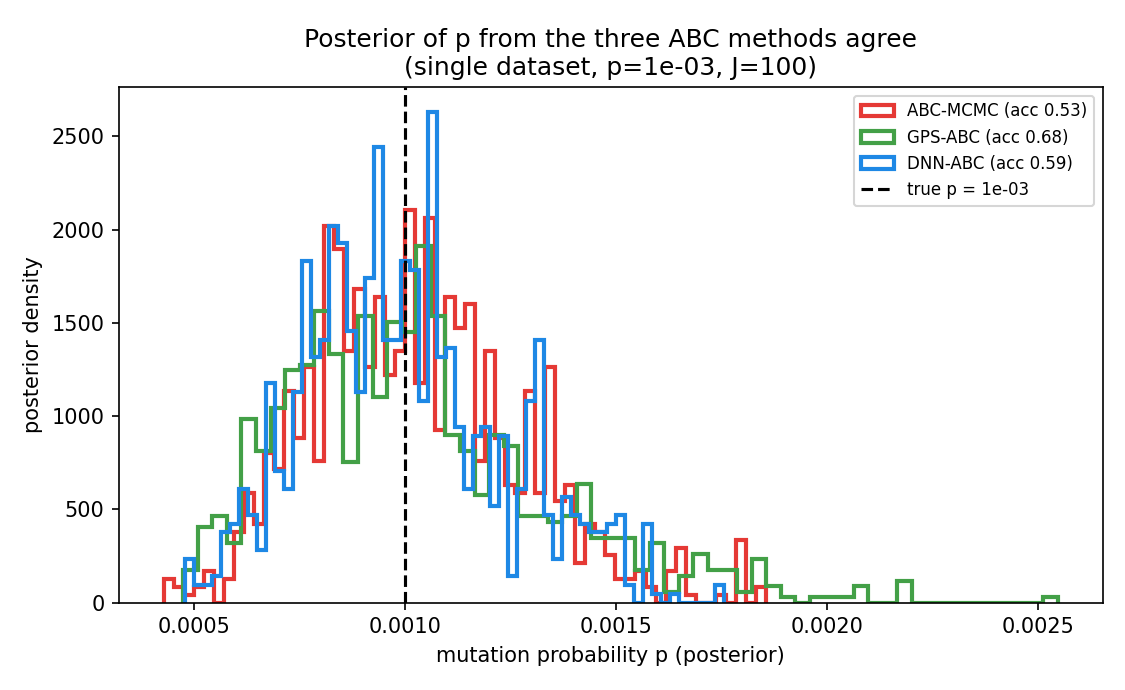
\includegraphics[width=0.85\linewidth]{Models/1D/results/figures/fig_posterior.png}
\caption{Study I: ABC-MCMC, GPS-ABC, and DNN-ABC posteriors for $\theta$ on a
single representative data set.}
\label{fig:posterior1D}
\end{figure*}

\subsection{Posterior coverage}
\label{sec:sim1D_coverage}

Split-conformal \emph{regression} calibration (Table~\ref{tab:fit1D}) is a
guarantee about the surrogate's predictive interval, not about whether the
downstream ABC credible interval brackets the true $p$ $95\%$ of the time.
Tables~\ref{tab:mse1D} and \ref{tab:ci1D} are silent on the second quantity, so
we save every credible interval's endpoints and measure it.


\begin{table*}[t]
\centering
\caption{Study I: empirical posterior coverage of the 95\% ABC credible
interval for $\hat p$, with binomial Monte Carlo standard error
($\sqrt{\hat c(1-\hat c)/R}$, $R=40$). This is a different quantity from
Table~\ref{tab:fit1D}'s regression coverage; see Section~\ref{sec:sim1D_coverage}.}
\label{tab:cov1D}
\begin{tabular}{rrrrr}
\toprule
$p$ & $J$ & ABC-MCMC & GPS-ABC & DNN-ABC \\
\midrule
$10^{-4}$ & 10  & 0.775 (0.066) & 0.825 (0.060) & 0.850 (0.056) \\
$10^{-4}$ & 50  & 0.900 (0.047) & 0.875 (0.052) & 0.900 (0.047) \\
$10^{-4}$ & 100 & 0.925 (0.042) & 0.950 (0.034) & 0.950 (0.034) \\
$10^{-3}$ & 10  & 0.800 (0.063) & 0.875 (0.052) & 0.875 (0.052) \\
$10^{-3}$ & 50  & 0.975 (0.025) & 0.975 (0.025) & 0.925 (0.042) \\
$10^{-3}$ & 100 & 0.950 (0.034) & 0.975 (0.025) & 0.925 (0.042) \\
$10^{-2}$ & 10  & 0.850 (0.056) & 0.875 (0.052) & 0.875 (0.052) \\
$10^{-2}$ & 50  & 1.000 (0.000) & 1.000 (0.000) & 0.925 (0.042) \\
$10^{-2}$ & 100 & 0.950 (0.034) & 1.000 (0.000) & 0.925 (0.042) \\
\bottomrule
\end{tabular}
\end{table*}

A surrogate trained only on $J=100$ summaries cannot know that a $J=10$
observation is noisier. Querying the $J{=}100$-only checkpoints at $J=10$ drops
GPS-ABC and DNN-ABC coverage to $0.43$--$0.53$, about half of nominal. The
$J$-specific surrogates of Table~\ref{tab:cov1D} recover most of that
shortfall: at $J=10$ they cover at $0.825$--$0.875$, one to three Monte Carlo
standard errors below nominal, and both reach or exceed nominal by $J=100$.
Neither surrogate is consistently the more under-covering, so
Table~\ref{tab:ci1D}'s length advantage for DNN-ABC is better evidence of real
precision than it would be if its intervals were also the least calibrated.
Separately, exact ABC-MCMC is itself below nominal at $J=10$ ($0.775$--$0.850$)
despite calling the true simulator at the correct $J$; this is a property of the
synthetic-likelihood kernel at this culture count, not of any surrogate.

The residual $J=10$ gap should not be explained away. Split-conformal calibration
is a marginal guarantee over the training distribution and does not size the
interval correctly at every $\theta$; the $J=10$ design is the smallest and
noisiest of the three. The practical lesson is that a surrogate's interval-length
advantage is not by itself evidence of equal calibration, and that training the
surrogate at the deployment condition is necessary, though not always
sufficient, for a trustworthy ABC posterior.

% =============================================================================
\section{Study II: The Two-Stage Mutation Model}
\label{sec:sim3D}
% =============================================================================

Study I holds $a=\delta=1$ and a single constant mutation probability. The
multi-parameter study of \citet{lu2023} is commonly read as that model with more
parameters freed, and it is not: it replaces the model with a \emph{two-stage}
(piecewise-constant) mutation rate,
\begin{equation}
p(t) \;=\;
\begin{cases}
p_1, & 0 < t \le \tau,\\[2pt]
p_2, & \tau < t \le t_p,
\end{cases}
\label{eq:twostage}
\end{equation}
in which the mutation probability jumps at an unknown time $\tau$. The
motivation is experimental: mutagenesis under sub-inhibitory antibiotic stress
involves a recovery step before plating, giving two distinct mutation regimes.
Study II estimates $(p_1, p_2, \tau)$ jointly, with $a=1$ throughout as in
\citeauthor{lu2023}. It is the main study of this paper, and it has two parts
that differ only in the parameter regime. Part A (Sections~\ref{sec:groundtruth3D}
to \ref{sec:sim3D_coverage}) uses a regime in which the exact simulator is feasible
($t_p=10$), so every method, including exact ABC-MCMC, can be compared. Part B
(Section~\ref{sec:sim3Dpub}) uses the regime of \citeauthor{lu2023}
($t_p=20$, $p\in[10^{-11},10^{-7}]$), reachable only with a fast simulator
that we first validate.

\subsection{Ground-truth data (Part A)}
\label{sec:groundtruth3D}

Ground truth comes from the exact, cell-by-cell simulator over a Latin
hypercube of $2{,}000$ design points in $(\log_{10}p_1, \log_{10}p_2, \tau)$
with ten replicates each: $20{,}000$ rows, $J=100$ cultures per row, $Z_0 = 1$,
$a = 1$, $t_p = 10$. A Latin hypercube replaces Study I's factorial grid because
a factorial design wastes points in three dimensions. Ranges are
$\log_{10}p_1, \log_{10}p_2 \in [-5,-1.3]$ and $\tau \in [0.1, 9.9]$. Fixing
$t_p$ at $10$ (about $2.2\times10^{4}$ cells per culture) rather than solving
for it per parameter as in Study I abandons the constant expected-mutant-count
design: the expected count ranges from $0.22$ to about $1{,}100$. Rates below
$\approx10^{-5}$ would leave almost every culture mutant-free at this $t_p$, so
the stated range keeps every design point informative; no row has $\dbar = 0$.

\noindent\textbf{The summary statistic is the fourth root.} \citeauthor{lu2023}
use $\sqrt{X/Z}$ for the constant-rate study but $\sqrt[4]{X/Z}$ for the
two-stage model, to make the response curve ``smooth and non-flat''. Study II
therefore takes
\[
  S \;=\; \frac{1}{J}\sum_{i=1}^{J} \left(X_i/Z_i\right)^{1/4},
\]
and every surrogate, baseline and sampler consumes $\log_{10}S$. Because the
ground truth stores each culture's $d_i = \sqrt{X_i/Z_i}$, $S$ is recovered
exactly as $\overline{\sqrt{d_i}}$ without re-simulating. The choice is
consequential: it lowers the surrogate's held-out error from $1.19\times$ its
irreducible floor to $1.11\times$ and changes which activation is selected
(Section~\ref{sec:sim3D_act}).

The port is validated by an exact degeneracy argument: setting $p_1 = p_2$
reduces Eq.~\eqref{eq:twostage} to the constant-rate model, and the two-stage
simulator then matches the constant-rate simulator in distribution. The full
dataset was generated in $23.6$ minutes ($39{,}227$ core-seconds, $92\%$
parallel efficiency on 30 cores).

\subsection{The inference problem is intrinsically asymmetric}
\label{sec:sim3D_identifiability}

Before any method is applied, the ground truth shows how much the scalar
summary can say about each parameter:

\begin{center}
\begin{tabular}{lccc}
\toprule
 & $p_2$ & $p_1$ & $\tau$ \\
\midrule
$\mathrm{corr}\!\left(\log_{10}S,\ \cdot\right)$ & $0.778$ & $0.337$ & $0.160$ \\
\bottomrule
\end{tabular}
\end{center}

$p_2$ is well determined, $p_1$ weakly, $\tau$ barely. The asymmetry is intrinsic
to the process: mutations arising before $\tau$ are exponentially rare because
few cells exist that early, so $p_1$'s contribution to the final mutant count is
swamped by $p_2$'s. \citeauthor{lu2023} report the same, describing multimodal
$p_1$ and $\tau$ marginals and attributing them to non-identifiability. A
fair evaluation must therefore report error per parameter, and on the
$\log_{10}$ scale: for a weakly identified parameter the posterior mean sits
wherever the prior puts its mass, so natural-scale RMSE diverges without
conveying anything.

\subsection{The surrogate, and why it is small}
\label{sec:arch3D}

The decisive measurement for this study is not a comparison between
architectures but the \emph{irreducible noise floor} of the data. The held-out
target is a two-replicate mean, so it carries $\mathbb{E}[\sigma^2]/2$ of
sampling noise no model can predict away. Here $\mathbb{E}[\sigma^2] =
6.90\times10^{-4}$, so the floor is $\mathrm{MSE} = 3.45\times10^{-4}$.
Table~\ref{tab:capacity3D} reports the architecture ladder against it.


\begin{table*}[t]
\centering
\caption{Study II: accuracy against the irreducible noise floor. MSE is measured
on held-out design-point means of $\log_{10}S$; the floor is
$3.45\times10^{-4}$. Three seeds per row.}
\label{tab:capacity3D}
\begin{tabular}{lrrrr}
\toprule
Hidden layers & Parameters & $\times$ floor & $R^2$ & \textmu s/query \\
\midrule
256--128--64 & 42{,}306 & 1.01 & 0.99681 & 56 \\
128--64 & 8{,}898 & 1.04 & 0.99671 & 42 \\
\textbf{64--32} (used) & \textbf{2{,}402} & \textbf{1.09} & \textbf{0.99656} & \textbf{40} \\
32--16 & 690 & 1.17 & 0.99628 & 37 \\
16--8 & 218 & 1.41 & 0.99553 & 38 \\
8--4 & 78 & 1.81 & 0.99426 & 37 \\
Linear (control) & 8 & 140.88 & 0.55319 & 29 \\
\bottomrule
\end{tabular}
\end{table*}

Two conclusions follow. First, a network is genuinely needed: the linear control
sits at $141\times$ the floor with $R^2 = 0.55$ (the fourth root makes the
surface harder for a linear model by nearly a factor of six relative to the
square root, so the choice of statistic strengthens the case for a network).
Second, capacity is not binding anywhere above roughly $700$ parameters: a
$690$-parameter network matches a $42{,}306$-parameter one within $17\%$, and a
$2{,}402$-parameter one within $8\%$. LayerNorm and residual depth were likewise
indistinguishable, as was the choice among common smooth activations
(Section~\ref{sec:sim3D_act}). This contrasts with Study I, where removing
BatchNorm changed accuracy by an order of magnitude; here capacity and depth buy
nothing, and a ranking among these variants would be reporting seed noise.

We select the architecture for parsimony, not accuracy or speed: a two-layer
$64\to32$ funnel with GELU/tanh activations, two output heads, and no BatchNorm.
Query latency is dominated by interpreter and framework overhead, so a $59\times$
reduction in parameters buys only about $29\%$ less latency.

\noindent\textbf{Does the tie survive downstream?} Table~\ref{tab:capacity3D} is a
curve-fit diagnostic. We test the same ladder on the ABC recovery task at
Table~\ref{tab:abc3D}'s own scale ($16$ replicates, all three truth triples,
$3{,}000$ iterations; \texttt{abc/run\_experiments\_capacity.py}), after a
two-replicate screen that every candidate survives.


\begin{table*}[t]
\centering
\caption{Study II: the capacity ladder's ABC-MCMC recovery, confirmed at
Table~\ref{tab:abc3D}'s own scale ($16$ replicates, all three truth triples,
$3{,}000$ MCMC iterations). $\Delta/\mathrm{SE}$ is each network's gap against
the deployed $64$--$32$, in combined Monte Carlo standard errors, maximized
over the nine parameter-by-truth cells.}
\label{tab:capacity3D_abc}
\begin{tabular}{lrrr}
\toprule
Hidden layers & Parameters & Mean $\mathrm{rmse}_{\log}$ & Resolved vs.\ deployed \\
\midrule
GP (GPS-ABC baseline) & --- & $0.990$ & --- \\
32--16 & $690$ & $1.067$ & $0/9$ (max $|\Delta/\mathrm{SE}|=1.63$) \\
128--64 & $8{,}898$ & $1.105$ & $0/9$ (max $|\Delta/\mathrm{SE}|=1.16$) \\
16--8 & $218$ & $1.133$ & $0/9$ (max $|\Delta/\mathrm{SE}|=1.06$) \\
64--32 (deployed) & $2{,}402$ & $1.142$ & --- \\
8--4 & $78$ & $1.149$ & $0/9$ (max $|\Delta/\mathrm{SE}|=1.32$) \\
256--128--64 & $42{,}306$ & $1.208$ & $0/9$ (max $|\Delta/\mathrm{SE}|=1.55$) \\
\bottomrule
\end{tabular}
\end{table*}

The tie survives. $32$--$16$ is again the best point estimate, but no pairwise
comparison against the deployed network is resolved at the $2$-MCSE level, not
even $256$--$128$--$64$ at $17\times$ the parameters, which is nominally the
worst of the six. Downstream accuracy is flat across more than two orders of
magnitude of parameter count. We do not redeploy on this evidence, since every
number in this paper is reported against the deployed $64\to32$ and the analysis
can show only that a smaller network is not measurably worse.

\noindent\textbf{Heteroscedasticity.} The variance head is not optional. The
within-design-point standard deviation of $\log_{10}\dbar$ varies by a factor
of $184$ across the design and correlates $-0.82$ with the target: where few
mutants arise, $\dbar$ is small and its relative scatter large. A GP's single
homoscedastic noise term cannot represent this, and because the acceptance step
consumes the predictive variance, an uncalibrated variance corrupts the
posterior even when the mean is exact.

\subsection{Choosing the activation function}
\label{sec:sim3D_act}

We compare ten activations spanning three families (piecewise-linear, smooth
saturating, smooth unbounded) on the deployed $64\to32$ network with five seeds
each, then the full $10\times10=100$ cross of layer-wise assignments, screened
on validation and confirmed on fifteen fresh seeds to avoid selection optimism
(Supplementary Material S2). The best-to-worst spread is $29\%$ of the best
row's MSE and softplus fails outright (strictly positive, so it cannot produce
centred activations), but the five leading candidates, GELU, tanh, LeakyReLU,
ReLU and Mish, are mutually indistinguishable. Selection optimism is real:
finalists perform on average $45\%$ of the confirmation table's spread worse on
fresh seeds than on the seeds that chose them, which is why evaluation never
reuses a selection seed. GELU into tanh is the best point estimate and the pair
we deploy, with held-out test MSE $1.06\times$ the floor. No conclusion turns on
this choice.

\subsection{Surrogate fit and calibration}
\label{sec:sim3D_fit}

The surrogate is trained on replicates 1--5, early-stopped and conformally
calibrated on 6--8, and evaluated on 9--10, so every design point appears in
every split and no parameter combination leaks. Each split is scored against its
own floor $\mathbb{E}[\sigma^2]/r$ for $r = 5, 3, 2$.


\begin{table*}[t]
\centering
\caption{Study II: surrogate fit. Each split is compared to its own irreducible
floor. Coverage is of the nominal-95\% predictive interval after a
split-conformal scale factor of $1.019$.}
\label{tab:fit3D}
\begin{tabular}{lrrrr}
\toprule
Split & $n$ & MSE (design means) & $\times$ its own floor & 95\% coverage \\
\midrule
Train (reps 1--5) & 10{,}000 & $1.60\times10^{-4}$ & 1.16 & 0.951 \\
Validation (6--8) & 6{,}000 & $2.95\times10^{-4}$ & 1.28 & 0.950 \\
\textbf{Test (9--10)} & \textbf{4{,}000} & $\mathbf{3.63\times10^{-4}}$ & \textbf{1.05} & \textbf{0.955} \\
\bottomrule
\end{tabular}
\end{table*}

The surrogate sits at its noise floor on all three splits, and the train and
test ratios ($1.16$ and $1.05$) are close enough that overfitting is not
detectable. The conformal scale factor of $1.019$ shows the variance head was
already almost calibrated before correction.


\subsection{ABC inference (Part A)}
\label{sec:sim3D_abc}

Inference is a random-walk Metropolis--Hastings sampler over the full vector
$\theta = (\log_{10}p_1, \log_{10}p_2, \tau)$, with component-wise truncated
proposals and Hastings corrections for the truncation: a genuine joint
three-parameter posterior, not a scalar inference with covariates. ABC-MCMC,
GPS-ABC and DNN-ABC share the sampler and differ only in how the statistic and
its uncertainty are obtained at each proposal, exactly as in Study I. MOM and
MLE have no counterpart here, since they assume a single mutation rate.

\noindent\textbf{Two Gaussian-process baselines.} Our GP is stronger than the one
\citeauthor{lu2023} use, and reporting only ours would overstate what the
published method achieves. Theirs fits an \emph{isotropic} squared exponential
to the untransformed rates $(p_1,p_2,\tau)$, predicting the untransformed
statistic, with one noise term. Ours uses one length scale per input, log-scaled
inputs and a learned white-noise term. The gap is large: on raw-scale fit the
reference configuration reaches $R^2 \approx 0.71$ while an otherwise identical
anisotropic kernel on the same $300$ design points reaches $\approx 0.99$, since
a single length scale cannot serve inputs whose ranges differ by a factor of
$\sim200$ ($p_1,p_2$ span $\approx 0.05$, $\tau$ spans $\approx 9.8$). Both are
fit from the same rows under the same budget, so the comparison isolates the
model. The reference performs ABC on the untransformed statistic, as its own
sampler does; ours works in $\log_{10}$.

\noindent\textbf{NPE.} Table~\ref{tab:abc3D} adds an amortized neural posterior
estimator. GPS-ABC and DNN-ABC learn a surrogate for the \emph{simulator} and
plug it into the ABC-MCMC sampler; NPE learns the \emph{posterior} directly, as
a conditional density $p(\theta \mid S)$, with no sampler in the loop. We train a
mixture-density network (\texttt{sbi}'s single-round NPE-C,
\citealp{tejerocantero2020}) once, offline, on the same $16{,}000$ rows DNN-ABC
trains on and the same fourth-root statistic. At inference it is queried once at
$S_{\mathrm{obs}}$ and returns posterior draws: no chain, acceptance step,
$\epsilon$ or per-observation re-simulation. It shares only the training budget
with the other surrogate methods; it is a different paradigm, not a fourth
variant. It belongs in this study because Section~\ref{sec:sim3D_identifiability}
establishes a well-identified parameter ($p_2$) and two poorly identified ones
within one jointly estimated posterior, the contrast that makes the comparison
informative.

Table~\ref{tab:abc3D} reports recovery over three truth triples with sixteen
replicates each, $3{,}000$ MCMC iterations and $1{,}000$ burn-in. Errors are
RMSE on the $\log_{10}$ scale for $p_1,p_2$ and absolute for $\tau$
(Section~\ref{sec:sim3D_identifiability}).


\begin{table*}[t]
\centering
\caption{Study II: joint recovery of $(p_1,p_2,\tau)$, averaged over three truth
triples, $J=100$, 16 replicates per cell. Errors are $\log_{10}$-scale RMSE for
$p_1,p_2$ (so $1.0$ means an order of magnitude) and absolute for $\tau$. Two
Gaussian-process baselines are reported: the strengthened one used throughout,
and one built to match the reference implementation of \citeauthor{lu2023}
(isotropic kernel, untransformed inputs and target). Exact ABC-MCMC (the
same synthetic-likelihood sampler Study I uses, calling the true simulator
$n_s=4$ times per iteration) is included as the expensive gold-standard
baseline. NPE has no acceptance
step, so its rate column reads ``---''.}
\label{tab:abc3D}
\begin{tabular}{llrrrr}
\toprule
Method & Parameter & RMSE & Mean 95\% CI width & Coverage & Accept.\ rate \\
\midrule
ABC-MCMC & $p_1$   & 1.403 & 3.33e-2 & 0.938 & 0.133 \\
(exact) & $p_2$   & 0.298 & 2.86e-2 & 0.896 & \\
        & $\tau$  & 1.847 & 8.71 & 1.000 & \\
\midrule
GPS-ABC & $p_1$   & 1.391 & 3.46e-2 & 1.000 & 0.371 \\
(strengthened) & $p_2$   & 0.156 & 3.22e-2 & 1.000 & \\
        & $\tau$  & 1.422 & 9.07 & 1.000 & \\
\midrule
GPS-ABC & $p_1$   & \textbf{1.309} & 3.47e-2 & 1.000 & 0.810 \\
(reference) & $p_2$   & 0.241 & 3.05e-2 & 1.000 & \\
        & $\tau$  & 1.799 & 9.01 & 1.000 & \\
\midrule
DNN-ABC & $p_1$   & 1.407 & 3.43e-2 & 0.938 & 0.143 \\
        & $p_2$   & 0.258 & 3.07e-2 & 0.979 & \\
        & $\tau$  & 1.753 & 8.64 & 1.000 & \\
\midrule
NPE & $p_1$   & 1.374 & 3.11e-2 & 1.000 & --- \\
        & $p_2$   & \textbf{0.089} & 2.92e-2 & 1.000 & \\
        & $\tau$  & \textbf{1.407} & 8.78 & 1.000 & \\
\bottomrule
\end{tabular}
\end{table*}

\noindent\textbf{NPE wins where the model identifies, and only there.} On $p_2$,
NPE's RMSE ($0.089$) beats every surrogate at every truth tested, never the
reverse, and the gap is resolved at the $2$-MCSE level in seven of nine
surrogate comparisons (all three against the reference GP, two of three each
against the strengthened GP and DNN-ABC; the remaining two are ties). On $p_1$
and $\tau$, NPE is a mix of ties and occasional wins and losses against each GP
variant. No method extracts information the statistic does not carry, and
Table~\ref{tab:abc3D} does not show NPE beating that ceiling. The asymmetry is
the finding: where the model identifies a parameter, learning the posterior
directly outperformed substituting a surrogate into the same ABC-MCMC kernel,
beyond replicate noise; where it does not, no method does better than another.
Training and per-dataset sampling cost are negligible (seconds to train,
milliseconds per dataset), so the comparison is about accuracy, not speed.

\noindent\textbf{The same holds against the exact simulator.} Table~\ref{tab:abc3D}'s
ABC-MCMC row is the same synthetic-likelihood sampler run on Study II's own
truths, not a cross-study comparison. Across all nine parameter-by-truth
comparisons NPE never loses to exact ABC-MCMC and wins five at the $2$-MCSE
level: $p_2$ at all three truths ($t=5.96$, $2.44$, $3.73$) and $\tau$ at two
($t=2.01$, $3.68$; the first only just past the threshold); the remaining four
are ties, all at $p_1$ or at $\tau$ for $t=7$. An amortized estimator trained
once on simulator draws thus matches or beats not merely a cheap surrogate but
the expensive exact sampler, exactly where the model identifies the parameter.

\noindent\textbf{The surrogates are tied.} With Monte Carlo standard errors on
every cell, DNN-ABC against the strengthened GPS-ABC gives seven ties among nine
parameter-by-truth comparisons, and the remaining two favour GPS-ABC: $p_2$ at
$(10^{-4}, 10^{-2}, 3)$, $+0.050 \pm 0.039$, and $\tau$ at $(2\times10^{-3},
8\times10^{-3}, 5)$, $+0.411 \pm 0.409$, both marginal. Study I found a
consistent interval-length advantage for the network and it would be natural to
expect it to carry over; it does not. When both surrogates fit the response
surface essentially perfectly relative to its own noise (Section~\ref{sec:arch3D}),
the surrogate has stopped being the bottleneck and downstream accuracy is set by
identifiability. A surrogate can only help where surrogate error limits the
answer: true in Study I, not here. Mean interval widths agree as well ($p_1$:
$3.43\times10^{-2}$ for DNN-ABC, $3.46\times10^{-2}$ for GPS-ABC).

\noindent\textbf{Coverage at fixed truths is not informative here.} Coverage of
the nominal $95\%$ interval is $0.938$--$1.000$ for DNN-ABC and $1.000$
throughout for both GPs. At sixteen replicates coverage moves in steps of
$1/16$, so DNN-ABC's $0.938$ on $p_1$ is one replicate fewer than the GP's, well
inside the per-cell MCSE ($\pm 0.08$); we claim no difference. More importantly,
every method, NPE included, covers $\tau$ at $1.000$, which is what a nearly
unidentified parameter looks like: the credible interval spans most of the prior
box and contains the truth by construction. A coverage of $1.000$ is therefore a
symptom of non-identifiability, not evidence of calibration. This is not a
failure of the surrogate's regression calibration, which is near-exact on held-out
data ($0.955$, Table~\ref{tab:fit3D}). Exact ABC-MCMC alone under-covers $p_2$
($0.896$; forty-three replicates of forty-eight against a nominal $45.6$, about
$1.2$ coverage MCSEs below $0.95$), probably from its own pilot-simulation
noise, though not resolved at this replicate count. Section~\ref{sec:sim3D_sbc}
replaces fixed-truth coverage with a diagnostic that does not saturate.

\noindent\textbf{The tolerance $\epsilon$ does not drive the over-coverage.} We
re-ran GPS-ABC, GPS-ABC-ref and DNN-ABC (NPE has no $\epsilon$) across a
$16\times$ range of $\epsilon$ around the fixed value, $0.0025$ to $0.04$, on the
same observations. GPS-ABC-ref is flat at coverage $1.000$. GPS-ABC and DNN-ABC
each dip slightly at the tightest $\epsilon$ (to $0.979$ and $0.958$ on $p_1$ and
$p_2$, pooled over $48$ replicates) and return to $1.000$ at the loosest, but no
movement resolves at the $2$-MCSE level (largest $|\Delta/\mathrm{SE}| = 1.44$).
Interval width grows by $15$--$20\%$ on $p_1$ and $p_2$ and a few percent on
$\tau$, the ordinary effect of a wider kernel. The over-coverage on $\tau$
survives an order-of-magnitude change in $\epsilon$ in either direction, which
points to identifiability, not the kernel.

\noindent\textbf{Replicate count.} Table~\ref{tab:abc3D_r40} reruns the four
methods that do not call the exact simulator inside their sampler at $R=40$,
matching Study I (exact ABC-MCMC stays at $R=16$; its validation already cost
several hours).


\begin{table*}[t]
\centering
\caption{Study II at $R=40$, matching Study I's replicate count: same four
methods, same three truth triples, same $16{,}000$-row training budget.
Compare against Table~\ref{tab:abc3D}'s $R=16$ figures directly: point
estimates move by noise, not by any qualitative change.}
\label{tab:abc3D_r40}
\begin{tabular}{llrrrr}
\toprule
Method & Parameter & RMSE & Mean 95\% CI width & Coverage & Accept.\ rate \\
\midrule
GPS-ABC & $p_1$   & 1.400 & 3.57e-2 & 0.983 & 0.372 \\
(strengthened) & $p_2$   & 0.160 & 3.22e-2 & 1.000 & \\
        & $\tau$  & 1.524 & 9.07 & 1.000 & \\
\midrule
GPS-ABC & $p_1$   & \textbf{1.311} & 3.45e-2 & 1.000 & 0.808 \\
(reference) & $p_2$   & 0.236 & 3.04e-2 & 1.000 & \\
        & $\tau$  & 1.807 & 9.02 & 1.000 & \\
\midrule
DNN-ABC & $p_1$   & 1.416 & 3.44e-2 & 0.925 & 0.143 \\
        & $p_2$   & 0.285 & 2.95e-2 & 0.950 & \\
        & $\tau$  & 1.869 & 8.65 & 0.983 & \\
\midrule
NPE & $p_1$   & 1.374 & 3.11e-2 & 1.000 & --- \\
        & $p_2$   & \textbf{0.088} & 2.93e-2 & 1.000 & \\
        & $\tau$  & \textbf{1.416} & 8.78 & 1.000 & \\
\bottomrule
\end{tabular}
\end{table*}

Every point estimate is within a few percent of its $R=16$ counterpart and both
findings survive more sharply resolved: DNN-ABC still never beats GPS-ABC at the
$2$-MCSE level (four of nine comparisons now resolved, up from two, all favouring
GPS-ABC) and NPE still never loses to a surrogate on $p_2$ (resolved in eight of
nine, up from seven). Tripling the replicate count sharpens the same picture.

DNN-ABC's acceptance rate is $0.143$ against $0.371$ for the strengthened GP and
$0.810$ for the reference GP, so the chains mix very differently at the shared
proposal scale and some of the DNN's disadvantage may be tuning rather than
method. The reference GP's high acceptance is itself informative: a flatter,
less discriminating surrogate accepts more freely. Per-method proposal tuning is
the obvious next step and is not attempted.

Study II, Part A is therefore a null result on the surrogate question and a
positive one on the modelling question. The neural surrogate matches, but does
not beat, a GP on downstream inference, because neither is the limiting factor.
What binds is identifiability: $\tau$ carries an RMSE of roughly $1.7$--$1.9$ time
units against a prior range of $9.8$, and $p_1$ is recovered no better than an
order of magnitude by any method.


\subsection{Calibration beyond fixed truths}
\label{sec:sim3D_sbc}

Coverage at a fixed truth cannot separate a well-calibrated posterior from an
uninformative one: an interval that spans the prior covers any truth. We
therefore evaluate calibration by simulation-based calibration
\citep{talts2018} over truths drawn from the sampler's own prior. For each of
$N=400$ truths $\theta^\ast$ drawn uniformly from the box, we simulate an
observation, compute each method's posterior, and record whether central
$50$, $80$ and $95\%$ intervals contain $\theta^\ast$, the rank of $\theta^\ast$
among the posterior draws, and the posterior contraction $1-\mathrm{Var}_{\mathrm{post}}
/\mathrm{Var}_{\mathrm{prior}}$ on the $(\log_{10}p,\tau)$ scale, the share of
prior variance the data remove. An exactly calibrated posterior has coverage
equal to its nominal level and uniform ranks whatever the identifiability, so
departures are findings about the method and contraction says how much
information each method extracts. The exact sampler is omitted, since $N=400$
posterior runs each calling the simulator are infeasible.

\begin{table*}[t]
\centering
\caption{Prior-averaged calibration (SBC), $N=400$ truths per regime. Coverage
of central $50/80/95\%$ intervals (binomial MCSE $\le0.025$); rank KS is the
$p$-value of a Kolmogorov--Smirnov test of rank uniformity; contraction is the
fraction of prior variance removed. Part B is discussed in
Section~\ref{sec:sim3Dpub}.}
\label{tab:sbc}
\small
\begin{tabular}{llrrrrr}
\toprule
Method & Param. & Cov.\ 50 & Cov.\ 80 & Cov.\ 95 & Rank KS $p$ & Contraction \\
\midrule
\multicolumn{7}{l}{\textit{Part A}} \\
GPS-ABC & $p_1$ & 0.422 & 0.715 & 0.890 & 0.108 & 0.210 \\
 & $p_2$ & 0.458 & 0.720 & 0.885 & 0.011 & 0.722 \\
 & $\tau$ & 0.463 & 0.802 & 0.953 & 0.076 & 0.102 \\
\addlinespace[1pt]
DNN-ABC & $p_1$ & 0.372 & 0.680 & 0.868 & 0.016 & 0.257 \\
 & $p_2$ & 0.430 & 0.695 & 0.853 & 0.011 & 0.780 \\
 & $\tau$ & 0.477 & 0.785 & 0.925 & 0.251 & 0.129 \\
\addlinespace[1pt]
NPE & $p_1$ & 0.458 & 0.708 & 0.873 & 0.062 & 0.236 \\
 & $p_2$ & 0.432 & 0.750 & 0.905 & 0.137 & 0.672 \\
 & $\tau$ & 0.505 & 0.785 & 0.920 & 0.042 & 0.113 \\
\midrule
\multicolumn{7}{l}{\textit{Part B}} \\
GPS-ABC & $p_1$ & 0.472 & 0.745 & 0.922 & 0.499 & 0.032 \\
 & $p_2$ & 0.672 & 0.850 & 0.945 & 0.000 & 0.838 \\
 & $\tau$ & 0.472 & 0.780 & 0.943 & 0.089 & 0.077 \\
\addlinespace[1pt]
DNN-ABC & $p_1$ & 0.458 & 0.728 & 0.890 & 0.124 & 0.083 \\
 & $p_2$ & 0.495 & 0.767 & 0.897 & 0.597 & 0.875 \\
 & $\tau$ & 0.458 & 0.782 & 0.930 & 0.453 & 0.090 \\
\addlinespace[1pt]
NPE & $p_1$ & 0.445 & 0.728 & 0.875 & 0.195 & 0.106 \\
 & $p_2$ & 0.485 & 0.752 & 0.938 & 0.395 & 0.903 \\
 & $\tau$ & 0.463 & 0.792 & 0.915 & 0.004 & 0.130 \\
\bottomrule
\end{tabular}
\end{table*}

Part A first. Contraction reproduces the identifiability ordering of
Section~\ref{sec:sim3D_identifiability} with no reference to any truth:
$0.67$--$0.78$ of the prior variance of $p_2$ is removed, $0.21$--$0.26$ for
$p_1$ and $0.10$--$0.13$ for $\tau$. Calibration, however, contradicts what
fixed-truth coverage suggested. Nominal $95\%$ intervals cover between $0.85$
and $0.95$, below nominal for every method on $p_1$ and $p_2$, and the
surrogate-in-MCMC methods are the worst on $p_2$ (DNN-ABC $0.853\pm0.018$,
GPS-ABC $0.885\pm0.016$) with NPE closest ($0.905\pm0.015$). Rank
uniformity is rejected at the $5\%$ level in four of the nine
method--parameter cells (DNN-ABC on $p_1$ and $p_2$, GPS-ABC on $p_2$, NPE on
$\tau$), where about half a rejection would be expected by chance. The $1.000$ coverage of $\tau$ at fixed truths was therefore an
artefact of non-identifiability, and the same methods that appeared uniformly
over-covering are, averaged over the prior, mildly overconfident. This
is not specific to the surrogates: NPE, which has no kernel and no surrogate,
under-covers $p_1$ ($0.873$) as well. We do not have a diagnosis beyond noting
that the shortfall is small and shared across structurally different estimators.


\subsection{Does architecture matter here?}
\label{sec:sim3D_arch}

The MLP treats its three inputs as an unordered feature vector. Whether an
architecture with a different inductive bias would do better is a natural
question, and we test it. \citet{radev2020}'s alignment principle predicts a
feedforward network should be at least as good, since the three inputs have
neither temporal order nor exchangeability. We compare a 1-D CNN, a GRU and an
LSTM against the deployed MLP on surrogate fit and on the full ABC recovery
task, with the same truths, replicates and iterations as Part A. Setup and
per-family tables are in Supplementary Material S3; code and checkpoints are in
the repository.

CNN1D ties the MLP on fit at $3.6\times$ its query cost; LSTM and RNN are
measurably worse ($+12.6\%$, $+20.6\%$ MSE). Across $54$ pairwise ABC-recovery
comparisons at the $2$-MCSE level, $91\%$ are ties and \emph{none} favours a new
family. Pooled coverage is $0.951$--$0.979$ for the four neural families, a
spread too small to support any calibration conclusion. Neither a spatial prior
(CNN1D) nor a temporal one (RNN, LSTM) improves on the architecture-agnostic MLP
for this input, consistent with \citet{radev2020}, and the surrogate used
throughout remains the plain heteroscedastic MLP.

\subsection{Scope of Part A}
\label{sec:sim3D_coverage}

Part A differs from \citeauthor{lu2023}'s Study II in three ways. First, $t_p=10$
rather than $20$, forced by the exponential cost of exact simulation. Second,
$\log_{10}p_1,\log_{10}p_2\in[-5,-1.3]$ rather than $[-11,-7]$; the two ranges
do not overlap, so Part A studies the same \emph{model} in a different and easier
regime and makes no numerical comparison with their Table~4. Part B closes this
gap. Third, the model has no $\delta$: the reference two-stage implementation
carries no differential mutant growth rate, so this is a three-parameter study
where theirs is four-dimensional. The simulator threads $\delta$ through so the
extension needs no rewrite.


\subsection{Study II, Part B: the published regime}
\label{sec:sim3Dpub}

Part A leaves one gap open: its parameter regime does not overlap the one
\citeauthor{lu2023} study, so it is not a reproduction of their two-stage
results. Their regime has $t_p=20$ and $\log_{10}p_1,\log_{10}p_2\in[-11,-7]$,
with $\tau\in[0.1,19.9]$ (and a fourth parameter, $\delta$, which we fix at
$1$). At $t_p=20$ a culture holds about $5\times10^{8}$ cells and the exact
simulator is out of reach, so Part B needs a fast simulator. We first show that
the one we had was wrong.

\subsubsection{A corrected fast simulator}
\label{sec:fastsim}

Our earlier extension of \citeauthor{lu2023}'s Algorithm~4 to two stages drew
the number of mutation events as $M=\mathrm{round}(Zp\,F(\tau))$ at Yule arrival
times, with geometric clone sizes. Tested against the exact simulator at
$t_p=10$, it disagreed everywhere: with $p_1=p_2=10^{-4}$ the mean mutant count
per culture was $11.2$ against $43.1$, and a two-sample Kolmogorov--Smirnov test
on the per-culture statistic rejected at every setting tried ($p<10^{-12}$).
There are two errors. First, each division of a wild-type cell yields two
daughters, each mutating independently, so mutation events arrive at rate
$2apW(t)$, not $apW(t)$; the expected mutant count is $2pa\,t_pe^{at_p}$, which
the exact simulator reproduces. Second, the exact simulator evaluates $p(t)$ at
each cell's own division time, so a daughter born at $s<\tau$ mutates at rate
$p_1$ only if its lifetime ends before $\tau$. That makes the mutation
probability a smooth function of $s$ and, for founders that mutated at $p_1$,
truncates their first lifetime, which enlarges their clones.

The replacement is a hybrid. Cells are simulated exactly up to $s_0=8$ time
units; each cell then alive founds an independent subtree whose final size is
drawn from the Yule law (so $Z$ is exact), whose wild-type members emit mutation
events as a Poisson process with intensity $2aGe^{-a(t_p-s)}q(s)$ given the
subtree size $G$, and whose mutant founders have first lifetimes drawn
conditionally on how they mutated. Event times come from inverting a closed-form
cumulative intensity. The cost is that of the exact stage, about
$e^{as_0}\approx3\times10^{3}$ cells per culture, independent of $t_p$.

We validate against the exact simulator at the only scales where both are
feasible, $t_p=10$ and $t_p=12$, choosing rates such that the expected number of
mutation events per culture, $2pZ$, spans $0.1$ to $100$, the same range as the
published regime. Across $12$ parameter settings (nine at $t_p=10$, three at
$t_p=12$; $12{,}000$ and $3{,}000$ cultures per simulator) the smallest KS
$p$-value is $0.015$, above the Bonferroni threshold of $0.004$, and the largest
KS distance is $0.020$ (Supplementary Table S7). The approximation is for small
rates: the Poisson event count and the neglect of wild-type depletion make it
suitable for $p\lesssim10^{-3}$ per daughter, which covers Part B by a wide
margin. Validity at $t_p=20$ itself rests on extrapolation in $2pZ$, since the
exact simulator cannot be run there.

\subsubsection{Design and results}

Ground truth is a $2{,}000$-point Latin hypercube over the published ranges with
ten replicates per point, $J=100$, generated by the fast simulator in $2.6$
minutes. A culture with no mutants
contributes $0$ to $S$; $2.1\%$ of rows have $S=0$ for all $100$ cultures, all
with $p_2<10^{-10}$. We treat $\log_{10}S$ as left-censored and floor it at
$-4.5$, half the smallest attainable nonzero value. The network, GP and NPE are
trained exactly as in Part A, with no re-tuning, and the sampler's proposal
scale is widened in proportion to the prior box.


Table~\ref{tab:abc3Dpub} reports recovery at three truth triples chosen as in
Part A (a large and an early or late jump, and a small jump),
$(10^{-10},10^{-8},5)$, $(10^{-10},10^{-8},14)$ and $(10^{-9},3\times10^{-9},10)$,
with $16$ replicates per truth for the surrogate methods. We add a GP with
$1{,}500$ design points, the initial design size of \citeauthor{lu2023}, so the
GP is not handicapped by the $300$-point budget of Part A. The exact-sampler
baseline calls the fast simulator inside the chain ($n_s=4$) and is run at
$8$ replicates per truth on the same observations because each chain takes
an hour or more; coverage at fixed truths is reported but, as in Part A, it
saturates and is read through Table~\ref{tab:sbc} instead.

\begin{table*}[t]
\centering
\caption{Study II, Part B (published regime): recovery of $(p_1,p_2,\tau)$
averaged over three truth triples, $J=100$. RMSE is on the $\log_{10}$ scale for
$p_1,p_2$ and absolute for $\tau$; width is the mean $95\%$ interval width as a
fraction of the prior range. Bold marks the lowest RMSE per parameter, not a resolved difference (see text).
GPS-ABC rows differ only in design size. The exact-sampler row uses the fast
simulator inside the chain and $8$ replicates per truth.}
\label{tab:abc3Dpub}
\begin{tabular}{llrrrr}
\toprule
Method & Parameter & RMSE & 95\% width / prior & Coverage & Accept.\ rate \\
\midrule
ABC-MCMC (fast sim.) & $p_1$ & 1.732 & 0.900 & 0.958 & 0.185 \\
 & $p_2$ & 0.236 & 0.371 & 0.958 &  \\
 & $\tau$ & 3.873 & 0.905 & 0.958 &  \\
\midrule
GPS-ABC (300) & $p_1$ & 1.729 & 0.943 & 1.000 & 0.759 \\
 & $p_2$ & 0.293 & 0.552 & 1.000 &  \\
 & $\tau$ & 3.524 & 0.952 & 1.000 &  \\
\midrule
GPS-ABC (1500) & $p_1$ & 1.739 & 0.943 & 1.000 & 0.722 \\
 & $p_2$ & 0.229 & 0.565 & 1.000 &  \\
 & $\tau$ & \textbf{3.225} & 0.950 & 1.000 &  \\
\midrule
DNN-ABC & $p_1$ & 1.694 & 0.922 & 1.000 & 0.217 \\
 & $p_2$ & 0.102 & 0.370 & 1.000 &  \\
 & $\tau$ & 3.483 & 0.930 & 1.000 &  \\
\midrule
NPE & $p_1$ & \textbf{1.679} & 0.896 & 1.000 & --- \\
 & $p_2$ & \textbf{0.056} & 0.527 & 1.000 &  \\
 & $\tau$ & 3.303 & 0.901 & 1.000 &  \\
\bottomrule
\end{tabular}
\end{table*}

\noindent\textbf{The network beats the Gaussian process where it can.} On the
well-identified $p_2$ DNN-ABC's RMSE is $0.102$ against $0.293$ for the
$300$-point GP and $0.229$ for the $1{,}500$-point GP. The gaps are resolved at
the $2$-MCSE level at all three truths against both GPs ($|\Delta/\mathrm{SE}|$
from $7.4$ to $11.0$ against the $300$-point GP and from $2.8$ to $8.1$ against
the $1{,}500$-point GP). Part A's tie does not carry over, and the cause is
visible in the surrogate fit (Table~\ref{tab:fitpub}): the network sits at
$1.05\times$ the noise floor, while the GPs sit at $1.51\times$ ($300$ points) and
$1.20\times$ ($1{,}500$ points). Quintupling the GP design closes part of the
gap, consistent with the introduction's argument about design size and cubic
cost, but it is still well short of the network. In Part B surrogate error binds, and a better
surrogate helps; in Part A it did not bind.

\begin{table}[t]
\centering
\caption{Study II, Part B: held-out surrogate fit against the irreducible noise
floor (two-replicate test target, floor $1.21\times10^{-2}$).}
\label{tab:fitpub}
\small
\setlength{\tabcolsep}{4pt}
\begin{tabular}{lrrr}
\toprule
Surrogate & MSE & $\times$ floor & Cov.\ 95\% \\
\midrule
DNN & $1.27\times10^{-2}$ & $1.05$ & $0.942$ \\
GP, $300$ points & $1.84\times10^{-2}$ & $1.51$ & $0.930$ \\
GP, $1{,}500$ points & $1.46\times10^{-2}$ & $1.20$ & $0.920$ \\
\bottomrule
\end{tabular}
\end{table}

\noindent\textbf{NPE is best on $p_2$ again, and the ceiling is unchanged.} NPE
reaches an RMSE of $0.056$ on $p_2$, resolved against both GPs at every truth
($|\Delta/\mathrm{SE}|$ from $6.9$ to $17.5$) and against DNN-ABC at one of
three truths ($3.1$; the other two are ties of $1.6$ and $1.5$, both favouring
NPE). On $p_1$ and $\tau$ nothing separates the methods consistently: $p_1$ is
recovered to within about $1.7$ orders of magnitude by every method, against a
prior range of four, and the error in $\tau$ simply tracks the distance of the
truth from the prior centre (about $6$ time units at $\tau=5$, $2.6$--$3.5$ at
$\tau=14$ and $0.8$--$1.8$ at $\tau=10$), as it does when a posterior mean sits
near the prior mean. Posterior contraction in the
prior-averaged calibration confirms this: $0.84$--$0.90$ of the variance of
$p_2$ is removed and $0.03$--$0.13$ of that of $p_1$ and $\tau$
(Table~\ref{tab:sbc}).

\noindent\textbf{Calibration over the prior.} The SBC rows of
Table~\ref{tab:sbc} for Part B refine the same message. The $300$-point GP
\emph{over}-covers $p_2$ ($0.672$ at the $50\%$ level, $0.850$ at $80\%$ and
$0.945$ at $95\%$; rank KS $p<0.001$) while removing less variance than the
network ($0.838$ against $0.875$) and NPE ($0.903$). Its coverage is obtained by
being less informative, a trade a coverage number alone cannot show. DNN-ABC
under-covers $p_2$ mildly ($0.897$ at $95\%$) and NPE is closest to nominal
($0.938$). On $p_1$ and $\tau$ the methods are mostly within two to three binomial MCSEs
($0.01$--$0.02$) of nominal, except that DNN-ABC and NPE under-cover $p_1$
($0.890$, $0.875$) and NPE under-covers $\tau$ ($0.915$).

\noindent\textbf{The exact sampler, and what it costs.} With the fast simulator
inside the chain, ABC-MCMC reaches $p_2$ RMSEs of $0.111$, $0.472$ and $0.126$ at
the three truths, at $60$--$102$ minutes per chain against $5$ seconds for
DNN-ABC and $0.04$ seconds for NPE (about a thousandfold). It is resolved
better than the $300$-point GP at two of three truths ($|\Delta/\mathrm{SE}|=7.5$,
$3.4$) and than the $1{,}500$-point GP at the same two ($3.0$, $2.8$), tied with
DNN-ABC at all three ($|\Delta/\mathrm{SE}|\le1.7$), and beaten by NPE at one truth
($2.5$; ties at the other two). The poor value of $0.472$ comes from one chain of
eight at $\tau=14$ that settles on a wrong mode ($p_2\approx5\times10^{-10}$,
acceptance rate $0.11$), the kind of failure expected from a synthetic likelihood
estimated from $n_s=4$ pilot simulations. With eight replicates it is not
resolved from the other chains, and we report it rather than drop it. A network
in the loop therefore matches the sampler it replaces on the identified
parameter at a thousandth of the cost, and the amortized NPE is as accurate as
either.



% =============================================================================
\section{Discussion}
\label{sec:discussion}
% =============================================================================

The two studies answer the question of Section~\ref{sec:intro} with a condition,
not a verdict. \emph{A surrogate improves an ABC inference only where surrogate
error is what limits it.} In Study I it is: a heteroscedastic network gives
tighter intervals than a GP and a flat query cost. In Study II, Part A, it is not:
both surrogates sit at the data's noise floor (Table~\ref{tab:capacity3D}), the
neural and GP surrogates tie in seven of nine comparisons, and accuracy is set by
what the single summary statistic identifies. In Part B the condition flips
again. The surface spans four decades, is zero-inflated and strongly
heteroscedastic, and a 300-point GP sits at $1.51\times$ the noise floor and a
1{,}500-point GP at $1.20\times$, against $1.05\times$ for the network; the
network then beats both GPs on $p_2$ at every truth tested. The same method is
neutral or decisive depending on the regime, and the noise-floor measurement
predicts which. That measurement is cheap, and we recommend making it before any
surrogate comparison.

The second finding concerns identifiability. In both parts of Study II the
statistic identifies $p_2$ and, at best, weakly $p_1$ and $\tau$. An NPE trained
directly on simulator draws, with no surrogate and no acceptance kernel, beats
every surrogate on $p_2$, matches or beats the exact sampler there, and does no
better than anything on $p_1$ and $\tau$. Two structurally unrelated estimators, a surrogate
substituted into an MCMC kernel and a density estimator trained once, agree on
where the ceiling sits, which is evidence that the ceiling belongs to the model
rather than to either method. A practical consequence is that a better emulator
cannot repair a weakly identified parameter; a richer summary statistic is the
lever, and the surrogate is not.

The third finding is about calibration. Split-conformal calibration is a strong,
distribution-free guarantee, and it holds to high precision for the surrogate's
regression problem (coverage $0.955$ in Part A, $0.942$ in Part B). It says
nothing about the coverage of the downstream posterior. At fixed truths, every
method covers $\tau$ at $1.000$, which reflects an interval spanning the prior,
not calibration. Averaged over truths drawn from the prior, the picture reverses
(Section~\ref{sec:sim3D_sbc}): all methods, including NPE, are mildly
overconfident, with $95\%$ intervals covering between $0.85$ and $0.95$ in
Part A, and fixed-truth coverage had concealed it. The guarantee does not
transfer from the regression to the posterior, and the two come apart here. We
therefore recommend simulation-based calibration over prior draws, together with
posterior contraction, as the routine check for any surrogate-based
likelihood-free sampler.

Two architectural lessons recur. In Study I the dominant factor was not the
activation function, a near-tie among reasonable choices, but the presence of
BatchNorm \citep{ioffe2015}: its per-minibatch statistics are counter-productive
for a smooth regression on a bounded, one-sided domain, and removing it improved
the fit eleven-fold. In Study II no architectural choice mattered, because every
candidate already sat at the noise floor, and convolutional and recurrent
families, which have nothing to find in three unordered parameters
\citep{radev2020}, did no better. The practical lesson is to let the symmetry of
the input choose the architecture family before any hyperparameter search.

\noindent\textbf{Limitations.} This is a simulation study under known ground
truth, with no application to real fluctuation-experiment data as in
\citet{lu2023}; a real-data application is the natural next step, since only it
can speak to misspecification. Study II's three truth triples at one culture
count do not exhaust the parameter space, although the SBC analysis averages over
the whole prior. Part B rests on a fast simulator validated against the exact one
at $t_p=10$ and $12$ and extrapolated to $t_p=20$ through the expected number of
mutation events; it assumes small rates and drops $\delta$, so the published
four-parameter model is not covered. The exact-sampler baseline in Part B calls
that same fast simulator and uses fewer replicates than the surrogate methods.
Study I uses $40$ replicates against \citeauthor{lu2023}'s $100$, and we report
Monte Carlo standard errors throughout so that unresolved differences are not
over-interpreted. The prior is bounded in both studies to keep the exact
simulator feasible inside the sampler. Finally, why the surrogate-based
samplers under-cover under prior-averaged calibration, and whether a kernel-side
correction restores nominal coverage, is left open.

% =============================================================================
\section{Reproducibility}
\label{sec:repro}
% =============================================================================

\noindent\textbf{Code and data.} All code, data, trained weights and the exact
configuration for every table and figure are in the public repository
\url{https://github.com/sletch1/DNN-ABC-mutation-rates}. The one-dimensional and
two-stage ground-truth data sets are committed as plain-text CSV files with
self-documenting headers, together with the exact simulator that generated them
and the reference implementation it was ported from. The Part B ground truth is
regenerated in under three minutes by the script
\texttt{generate\_design\_published\_regime.py}.

\noindent\textbf{Environment.} All code is Python (\texttt{numpy}, \texttt{pandas},
\texttt{scipy}, \texttt{matplotlib}, \texttt{scikit-learn} for the GP baseline,
\texttt{torch} for the surrogates, \texttt{sbi} for NPE; minimum versions are
pinned in \texttt{requirements.txt}). No GPU is required; every model trains on
CPU in seconds to minutes.

\begin{sloppypar}
\noindent\textbf{Running it.} Each study has a single entry point,
\texttt{run\_all.py}, that retrains its surrogate, reproduces its ABC tables,
recomputes Monte Carlo standard errors and regenerates every figure. It asks at
the console whether to run a short pipeline check or the full settings, and runs
under any Python interpreter. The individual steps are documented in each
package's guide, in the order of this paper. Study II's default run trains NPE
inline. Its exact ABC-MCMC row is the one result \texttt{run\_all.py} does not
reproduce by default because it takes several hours; \texttt{abc/add\_exact.py}
backfills it, and the third menu option reruns everything including it. The
$\epsilon$ sweep (\texttt{abc/eps\_sweep.py}), the $R=40$ check
(\texttt{run\_experiments.py --reps 40 --no-sim}), the prior-averaged calibration
(\texttt{abc/calibration\_sbc.py --regime main|published}) and Part B
(\texttt{abc/run\_published\_regime.py}, with
\texttt{tests/validate\_fast\_simulator.py} for the simulator check) are each one
additional command.
\end{sloppypar}

\noindent\textbf{Validation scripts.} \texttt{tests/validate\_simulator.py}
re-derives, rather than asserts, that the two-stage exact simulator reduces to the
constant-rate one in both degenerate limits, checked in distribution by a
two-sample test. The summary statistic is recomputed from the stored per-culture
values, so the choice of root is a single switch that cannot drift between the
surrogate, the baselines and the sampler. Every number in the tables and in the
architecture-family comparison is produced by these scripts directly from the
committed data, with no manual post-processing, and the Monte Carlo standard
errors are computed from the per-replicate output each script already writes.

% =============================================================================
\section{Conclusion}
\label{sec:conclusion}
% =============================================================================

A heteroscedastic neural surrogate, calibrated by split-conformal prediction and
substituted for the Gaussian process inside \citeauthor{lu2023}'s ABC-MCMC
sampler, gives tighter intervals at matched accuracy and a $68$ to $2{,}381$-fold
speedup over the exact sampler in the one-dimensional benchmark. In the
two-stage model, which is the main study, the picture is conditional. Where a GP
already reaches the data's noise floor (Part A) the surrogates tie and
identifiability decides accuracy: $p_2$ is recovered well, $p_1$ and $\tau$
barely. Where the response surface is harder (Part B, the regime of the published
study, made reachable by a corrected and validated fast simulator) the network is
clearly better than the GP, even against a GP five times larger. In both,
an amortized NPE trained on the same simulations matches or beats every surrogate
and the exact sampler on the identified parameter and cannot exceed the
identifiability ceiling on the others.

The general lessons are three. Measure the noise floor before comparing
architectures or surrogates, because it predicts whether a comparison can report
anything. Do not read a surrogate's regression calibration as the calibration of
the posterior built on it, and check the latter with simulation-based calibration
over prior draws and posterior contraction, because fixed-truth coverage saturates
at one for weakly identified parameters. And do not expect a better emulator to
repair a parameter the data do not identify. These conclusions should apply
beyond this model to ABC procedures built on a regression surrogate for an
expensive simulator.

% =============================================================================
\backmatter

\section*{Declarations}

\bmhead{Data availability}
The ground-truth data sets analysed in this study (Section~\ref{sec:sim1D}
for the one-dimensional constant-rate model and Section~\ref{sec:groundtruth3D}
for the two-stage model) are committed as plain-text CSV files in the code
repository accompanying this paper, \url{https://github.com/sletch1/DNN-ABC-mutation-rates}.
[PLACEHOLDER: insert the specific release tag or archived-version DOI
corresponding to this submission once one has been minted.]

\bmhead{Code availability}
All code used to produce the results in this paper (surrogate training,
ABC-MCMC sampling, Monte Carlo standard error computation, and figure/table
generation) is available in the same repository as above,
\url{https://github.com/sletch1/DNN-ABC-mutation-rates}. A single entry
point per study, \texttt{run\_all.py} (see Section~\ref{sec:repro}),
reproduces the full pipeline in one command. [PLACEHOLDER: insert the
release tag or archived-version DOI corresponding to this submission once
one has been minted.]

\bmhead{Competing interests}
[PLACEHOLDER: the authors will state any competing interests here prior to
submission.]

\bmhead{Funding}
[PLACEHOLDER: the authors will state funding sources, if any, here prior to
submission.]

\bmhead{Author contributions}
[DRAFT, please confirm or edit before submission: S.L. conceived and
implemented the surrogate methods, ran all simulation studies and analyses,
and wrote the manuscript. H.Z. and X.W. supervised the research and
critically reviewed the manuscript. All authors read and approved the final
manuscript.]

% =============================================================================
\bibliography{manuscript}

\end{document}

